\section{Background and Motivation}
\label{sec:example}
Control theoretic designs provide formal guarantees that systems
achieve desired behavior despite dynamic environments. For example, a
car's cruise control regulates fuel flow into the engine to maintain
the driver's desired speed despite changes in wind condition, road
condition, incline, tire pressure, and many other details.  In fact,
those details are not incorporated into the cruise control model at
all; instead, the controller uses a difference model that relates the
current speed to the past speed and the past fuel
flow.\footnote{Continuous time systems would use \emph{differential}
  equations, but since computer systems are discretized we restrict
  ourselves to \emph{difference} equations.}

We present a brief example using control theory to provide reliable
performance to the LAVAMD application running on a heterogeneous ARM
big.LITTLE architecture with four big cores and four LITTLE cores.
Our goal is to maintain application-specified performance despite
unpredictable events such as another application entering the system
and competing for resources.  We show how this problem is a
straightforward application of control theory when the only
controllable resource is clockspeed, but the complexity jumps
dramatically when we consider available cores, core types, and
clockspeed together.

\PUNT{We first show how this problem can be a straightforward
  application of classic control techniques if we only consider
  clockspeed as the controllable resource.  We then show how the
  problem's complexity jumps dramatically when we consider not only
  clockspeed but allocating combinations of big and LITTLE cores.
  While this more complex problem is solvable using advanced control
  techniques, the solutions require {\em a priori} models of the
  applications' response to configurations of big and LITTLE cores and
  their respective frequencies.\TODO{cite??}  We conclude by arguing
  for a combination of control theory and machine learning that
  provides control theoretic performance guarantees without requiring
  {\em a priori} models of the controlled application.}

\subsection{Controlling Clockspeed}
\begin{figure}
  \subfloat[]
  {
    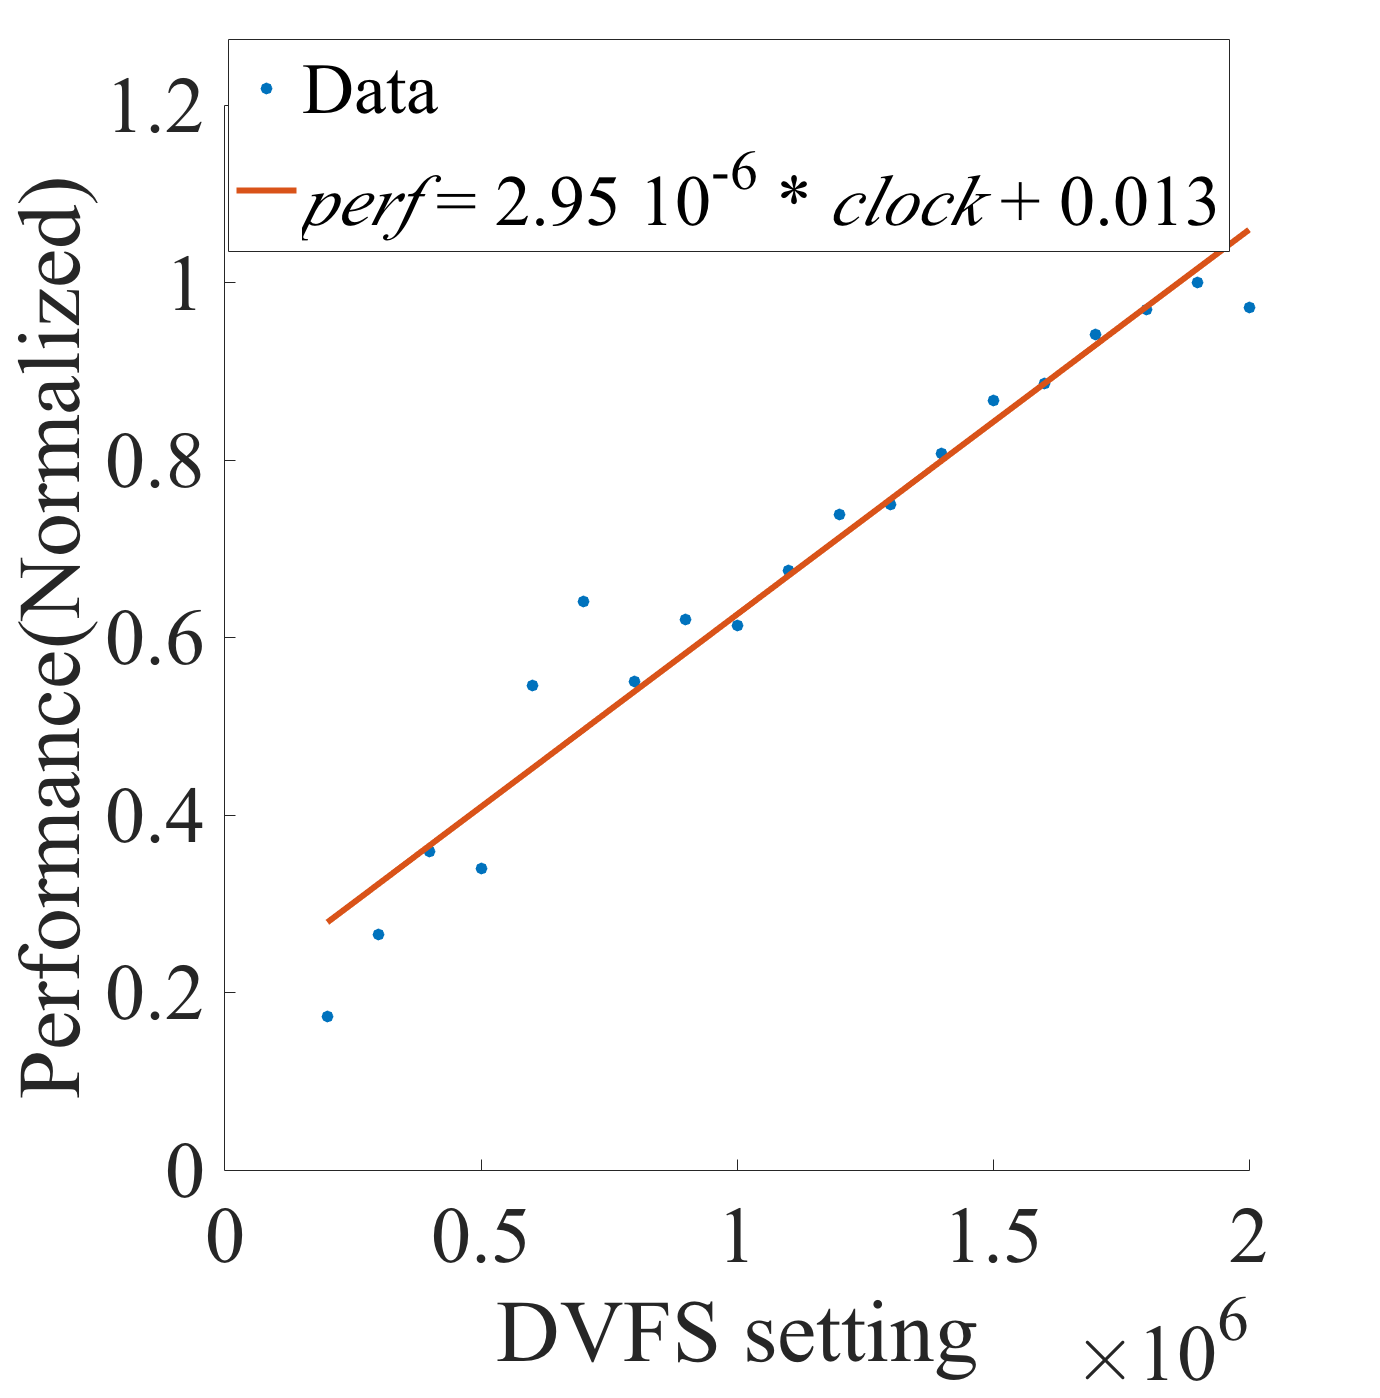
\includegraphics[width=.25\textwidth]{figures/lavamd_dvfs.png}
    \label{fig:lavamd_model}
  }
  \subfloat[]
  {
    \begin{tikzpicture}
\begin{centering}

\definecolor{s1}{RGB}{228, 26, 28}
\definecolor{s2}{RGB}{55, 126, 184}
\definecolor{s3}{RGB}{77, 175, 74}
\definecolor{s4}{RGB}{152, 78, 163}
\definecolor{s5}{RGB}{255, 127, 0}

\begin{groupplot}[
    group style={
        group name=plots,
        group size=1 by 1,
        xlabels at=edge bottom,
        xticklabels at=edge bottom,
        vertical sep=5pt
    },
height=4.1cm,
width=0.45\columnwidth,
xmajorgrids,
ymajorgrids,
grid style={dashed},
xmin=0,
xmax=20,
yticklabel pos=left,
enlargelimits=false,
tick align = outside,
tick style={white},
xticklabel shift={-5pt},
yticklabel shift={-5pt},
ylabel shift={-2pt},
ylabel style={align=center},
unbounded coords=jump,
]

\nextgroupplot[ylabel={\scriptsize Performance (Normalized)}, % Performance
%xtick={0,500,1000,1500,2000,2500,3000,3500,4000,4500},
ytick={0.0,0.5,1.0,1.5,2.0},
yticklabels={,0.25,0.5,1.0,1.5},
%xtick={0,30,60,120,160,200,240,280,320,480},
%xticklabels={,0,30,60,120,160,200,240,280,320,480},
%yticklabel style={font=\footnotesize},
xlabel={\footnotesize Iteration},
ymin=0,
ymax=1.5,
legend entries={,{\scriptsize $\mathsf{Uncontrolled}$},{\scriptsize $\mathsf{Controlled}$}},
legend style={fill=none,draw=none,at={(0.5,1.4)},anchor=north,legend columns=1,
line width=3pt},
]
\addplot[thick, dashed, black] coordinates {(10,0) (10,1.5)};
\addplot[thick, solid, color=s4] table[x index=0,y index=1,col sep=tab] {img/image_text/kmeans-example.txt};
\addplot[thick, solid, color=s5] table[x index=0,y index=2,col sep=tab] {img/image_text/kmeans-example.txt};

%\addplot[thick, dashed, black] coordinates {(130,0) (130, 2)};
\end{groupplot}
\end{centering}

\end{tikzpicture}

    \label{fig:lavamd_control}
  }
 \label{fig:freq-control}
 \caption{LAVAMD's performance is linear in DVFS setting (a) making it
   easy to control even when another application interferes (b).}
\end{figure}

We would like to construct a controller that adjusts processor
frequency to ensure that a performance goal is met
\cite{lefurgy2008power}.  As \figref{fig:lavamd_model} demonstrates
that it is quite simple to map clock frequency to LAVAMD performance.
we can see that the data follows a fairly linear fit. Our simplest
form of controller simply measures the error between the desired
application performance and current performance, divides by the slope
of the linear fit, and then adds that to the previous frequency --
just like the cruise control in the car.  This process repeats at
discrete time intervals The process repeats at discrete time
intervals, allowing the controller to adjust to harder or easier
phases of LAVAMD and to adjust to external events.

We demonstrate this ability to adapt to dynamics in
\figref{fig:lavamd_control}.  Suppose, the $goal$ performance is 0.5,
meaning that we are happy achieving 50\% of the maximum possible
performance. After 10 iterations, we launch a second application on a
single big core and it competes for resources.
\figref{fig:lavamd_control} shows LAVAMD's behavior in this scenario
when we run both without and with a controller.  Without a controller,
the system maintains the original clockspeed necessary to hit the
target, but that speed is no longer sufficient.  In contrast, even
though the controller does not have a model of application
interference it detects the difference in speed and adjusts the
frequency up to return LAVAMD to the desired performance. In fact,
even this simple controller provides formal guarantees that it will
converge to the desired performance after external changes like the
one we introduced here \cite{Hellerstein2004a}.

\PUNT{
We can use the same approach to construct a controller that adjusts
processor frequency to ensure that a performance goal is met
\cite{lefurgy}.  While it is statically quite simple to map clock
frequency to program performance, we want to build a system that
constantly adjusts frequency to maintain performance even if resource
availability changes or the application input changes. 

We can profile the application running
on all four big cores and a number of frequencies to determine the
relationship between frequency setting and performance as shown in
\figref{fig:lavamd_model}.  By fitting a line to this data we obtain
the model:
\begin{equation}
  perf(t) = 2.95 \times 10^{-6} \cdot clock(t-1) + \delta \label{eqn:clock}
\end{equation}
This model states the observed $perf(t)$ is some constant (the slope
of our model) times the clockspeed applied at the previous time step,
$clock(t-1)$, plus some noise, $\delta$ drawn from a Gaussian
distribution.  This simple linear difference model ignores low-level
details like instruction mix, and instead uses feedback, predicting
behavior of the next time step as a function of the previous time
step.  Using the relationship of \eqnref{clock}, we synthesize a
simple controller that is provably convergent to the performance
$goal$ performance \cite{ICSE2014}:
\begin{eqnarray}
  error(t) &=& goal - perf(t) \label{eqn:clock-error} \\
  clock(t) &=& clock(t-1) - \frac{error(t)}{ 2.95 \times 10^{-6}}
  \label{eqn:clock-control}
\end{eqnarray}




\subsection{Benefits of Control}
To demonstrate the benefits of applying control to manage LAVAMD's
performance, we run it in an unpredictable environment.  The $goal$
performance is 0.5, meaning that we are happy achieving 50\% of the
maximum possible performance. After 10 iterations, we launch a second
application on a single big core and it competes for resources.
\figref{fig:lavamd_control} shows LAVAMD's behavior in this scenario
when we run both without and with a controller.  Without a controller,
the system maintains the clockspeed necessary to hit the target, but
that speed is no longer sufficient.  In contrast, even though the
controller does not have a model of application interference it
detects the difference in speed and adjusts the frequency up to return
LAVAMD to the desired performance. In fact, the simple controller in
\eqnsref{clock-error}{clock-control} provides formal guarantees that
it will converge to the desired performance after external changes
like the one we introduced here \cite{Hellerstein2004a}.  
}

\begin{figure}
  \subfloat[]
  {
    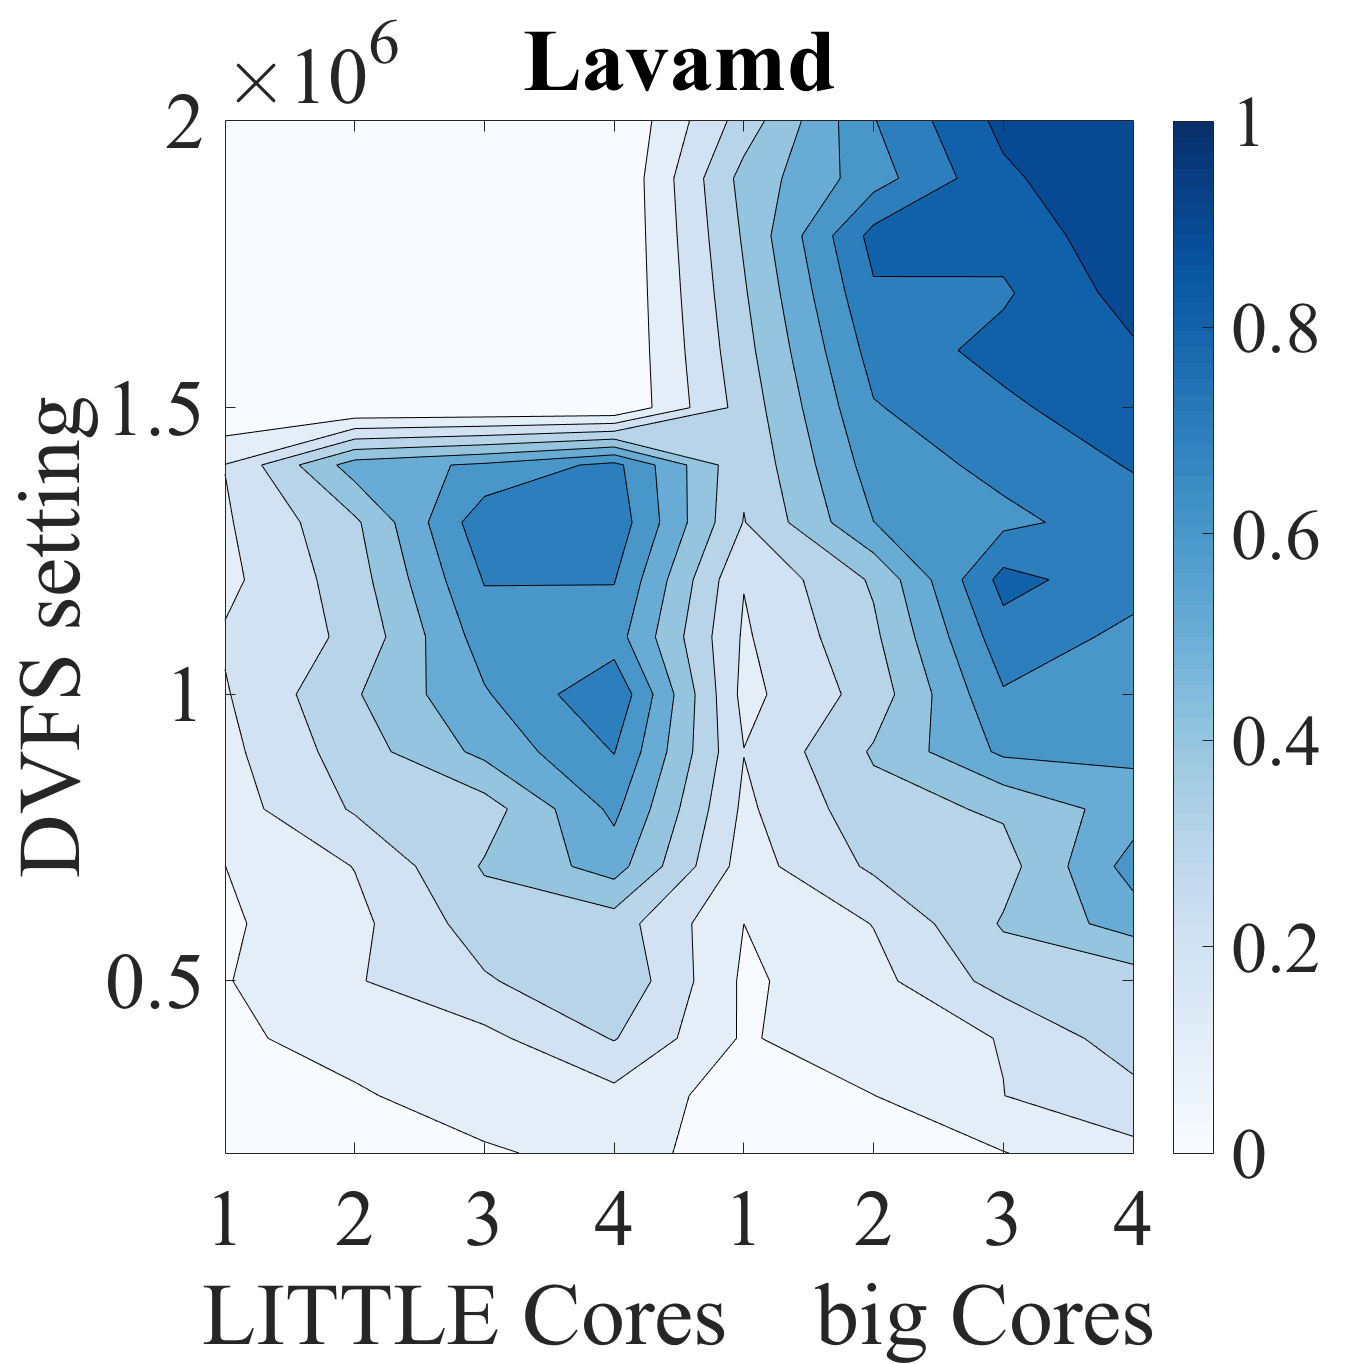
\includegraphics[width=.25\textwidth]{figures/lavamd.png}
    \label{fig:lavamd_contour}
  }
  \subfloat[]
  {
    \begin{tikzpicture}
\begin{centering}

\begin{groupplot}[
    group style={
        group name=plots,
        group size=1 by 1,
        xlabels at=edge bottom,
        xticklabels at=edge bottom,
        vertical sep=5pt
    },
height=4.1cm,
width=0.45\columnwidth,
xmajorgrids,
ymajorgrids,
grid style={dashed},
xmax=20,
yticklabel pos=left,
enlargelimits=false,
tick align = outside,
tick style={white},
xticklabel shift={-5pt},
yticklabel shift={-5pt},
ylabel shift={-2pt},
ylabel style={align=center},
unbounded coords=jump,
]

\nextgroupplot[ylabel={\scriptsize Performance (Normalized)}, % Performance
xlabel={\footnotesize Iteration},
ytick={0.0,0.5,1.0,1.5,2.0},
yticklabels={,0.25,0.5,1.0,1.5},
legend entries={,{\scriptsize $\mathsf{Generic~Model}$},{\scriptsize $\mathsf{LAVAMD model}$}},
legend style={fill=none,draw=none,at={(0.5,1.4)},anchor=north,legend columns=1,line width=3pt},
]

\addplot[thick, dashed, black] coordinates {(10,0) (10,1.5)};
\addplot[thick, solid, color=poet] table[x index=0,y index=1,col sep=tab] {img/image_text/lavamd-example.txt};
\addplot[thick, solid, color=cal] table[x index=0,y index=2,col sep=tab] {img/image_text/lavamd-example.txt};
\end{groupplot}
\end{centering}
\end{tikzpicture}
    \label{fig:lavamd_control2}
  }
  \caption{LAVAMD's performance is non-convex when considering all
    resources in the ARM big.LITTLE (a) making it difficult to control
    with a generic model (b).}
 \label{fig:learning-models}
\end{figure}


\subsection{Controlling a Heterogeneous System}
The simple system described above has its limitations; first, it only
works for clockspeed, but our test system also has different core
types.  We could save substantial energy by controlling application
performance with a combination of frequency and core scheduling
\cite{Carroll2013,kim-cpsna}.  When we consider core number, core
type, and frequency we get a much more complicated relationship with
performance. \figref{fig:lavamd_contour} shows that, for LAVAMD, the
relationship between a resource \emph{configuration} -- \ie{} an
assignment of resources -- and performance is non-convex -- \ie{}
there are multiple local maxima.

\PUNT{The combination of non-convexity and non-linearity is usually dealt
with in two steps. First, we find the convex hull of the tradeoff
space.  Second, we build several linear controllers and use their
combination to approximate the non-linear response.  This process of
dealing with complicated interactions between resources is one of the
difficulties of controlling computing systems.  }

Several different approaches have addressed this issue by:
specializing control for a particular platform and class of
application \cite{grace,Agilos,METE}, automatically synthesizing
controllers \cite{josep-isca2016,FSE2015}, or building control
libraries that users specialize by providing appropriate models
\cite{POET,ControlWare,SWiFT}. These approaches have two related
drawbacks.  First, all require prior knowledge of the application and
systems under control; while control theoretic designs provide formal
guarantees of their behavior, those guarantees are predicated on the
control models being known {\em a priori}. Second, since these
approaches require the models to be known ahead of time, they create
specialized controllers that are appropriate only for the given
application-class and system for which the model applies.  

\PUNT{This
  specialization can clearly be seen in \eqnref{clock-control}, as the
  model parameter appears directly in the definition of the control
  system.  If new applications arise that have a different response to
  the same resources, a new controller will have to be designed and
  implemented.}

We illustrate this problem in \figref{fig:lavamd_control2}.  We again
attempt to control LAVAMD to deliver reliable performance at 50\% of
the maximum achievable.  This time we use two different control
models, the first is a general control model representing average
response to resources across a number of test applications.  The
second model is specific to LAVAMD.  The general model produces wildly
oscillating performance, alternating between using all big cores at
the highest frequency and one little core at a low frequency.  In
contrast, the LAVAMD-specific model provides perfectly steady control.
In addition, the steady model provides much greater energy savings
(over 3$\times$) because it uses a combination of big and LITTLE cores
to meet the performance target, while the general model ends up
running all the big cores at maximum speed about half the time.

\PUNT{
\subsection{Motivation}
In this section we have seen the benefits and drawbacks of applying
control to computing systems:
\begin{itemize}
\item {\bf Benefit:} Provides provably reliable performance with
  formal guarantees that that performance will be met.
\item {\bf Drawback:} Both the empirical and formal behavior of the
  system are predicated on models that must be known in advance and
  are not generally applicable.
\end{itemize}

Our goal in this paper is to \emph{design and implement a system that
  provides both empirical and analytical guarantees of convergence to
  performance goals, even when working with new application without a
  priori knowledge of their behavior.}  To accomplish this goal we
combine control theory with machine learning by:
\begin{itemize}
\item Creating a generalized control design for resource management
  that accepts any model at runtime.
\item Offloading expensive learning techniques to a remote server that
  aggregates data from multiple applications and devices to quickly
  and accurately learn models of new applications.
\item Creating an interface that allows those models to be sent from
  the server to local devices and accessed efficiently
\item Combining statistical and control theoretical formal analysis to
  show that the system will converge to the desired performance.
\end{itemize}
The next section details how we accomplish these objectives.
}
